\section{Sơ bộ}
\subsection{Tính chất của đồ thị con và đồ thị phân chia}

\begin{lemma}
    \label{lem:plnp}
    Đồ thị con của đồ thị phẳng là đồ thị phẳng
\end{lemma}

\begin{proof}
    Nếu $G$ là đồ thị phẳng, nghĩa là tồn tại một biểu diễn phẳng của $G$. Với mọi đồ thị con
    $H$ của $G$, ta có thể tìm đươc các đỉnh và cạnh của $H$ trong biểu diễn phẳng của $G$.
    Từ đó, ta dựng được một biểu diễn phẳng của $H$.
\end{proof}


\begin{lemma}
    \label{lem:subp}
    Đồ thị phân chia của một đồ thị không phẳng là một đồ thị không phẳng.
\end{lemma}
\begin{proof}
    Giả sử đồ thị không phẳng $G$ có một đồ thị phân chia $G'$ của $G$ là đồ thị phẳng.
    Khi ta xóa đỉnh được thêm bởi phép \hyperref[def:subdivision]{\textit{chia nhỏ}} và dựng lại cạnh ban đầu (không thay đổi hình dạng và vị trí của các đường đi). Ta thu được biểu diễn phẳng của $G$, vô lý.
    Vậy nên, nếu $G$ không phẳng thì các đồ thị phân chia của $G$ cũng không phẳng.
\end{proof}

\subsection{Tính chất đồ thị 2-liên thông}
\begin{corollary}
    Xóa một đỉnh khỏi đồ thị 2-liên thông không làm mất tính liên thông của nó.
\end{corollary}
\begin{proof}
    Vì đồ thị $G$ là 2-liên thông nên $\kappa(G) \geq 2$. Nếu việc loại bỏ 1 điểm khỏi $G$ làm nó mất tính liên thông nghĩa là $\kappa(G) \leq 1$. Vô lý.
\end{proof}

\begin{lemma}
    Đồ thị 2-liên thông khi và chỉ khi mọi cặp đỉnh trong đồ thị đều có một chu trình đi qua chúng.
    \begin{proof}
        $(\Rightarrow)$ Cho $G$ là đồ thị 2-liên thông, ta sẽ chứng minh bằng quy nạp, mọi cặp đỉnh $u,v \in V(G)$ đều có một chu trình đi qua chúng.

        Ta định nghĩa \textit{khoảng cách} giữa $u$ và $v$ là độ dài đường đi ngắn nhất giữa $u$ và $v$

        \begin{itemize}
            \item Trường hợp cơ bản: $u$ kề $v$ ($u,v$ có \textit{khoảng cách} là 1)
                  \begin{center}
                      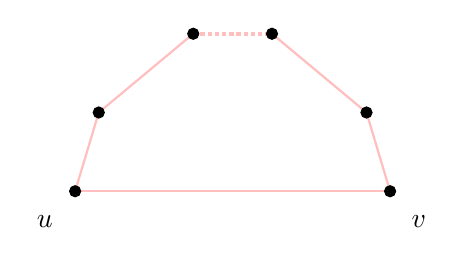
\begin{tikzpicture}
                          \draw[pink, thick] (0,0) -- (0.3,1);
                          \draw[pink, thick] (0.3,1) -- (1.5,2);
                          \draw[densely dotted, pink, ultra thick] (1.5,2) -- (2.5,2);
                          \draw[pink, thick] (2.5,2) -- (3.7,1);
                          \draw[pink, thick] (3.7,1) -- (4,0);
                          \draw[pink, thick] (0,0) -- (4,0);
                          \node at (0,0,1) {$u$};
                          \node at (4.75,0,1) {$v$};
                          \filldraw[black] (0,0) circle (2pt);
                          \filldraw[black] (0.3,1) circle (2pt);
                          \filldraw[black] (1.5,2) circle (2pt);
                          \filldraw[black] (2.5,2) circle (2pt);
                          \filldraw[black] (3.7,1) circle (2pt);
                          \filldraw[black] (4,0) circle (2pt);
                      \end{tikzpicture}
                  \end{center}
                  Nếu không có đường đi giữa $u$ và $v$ không chứa cạnh $uv$ thì $u$ hoặc $v$ sẽ là đỉnh cắt, dẫn đến $\kappa(G) \leq 1$.
                  Vậy nên tồn tại đường đi khác giữa $u$ và $v$ mà không chứa cạnh $uv$, kết hợp với cạnh $uv$ sẽ tạo thành một chu trình chứa $u,v$.

            \item \indent Giả sử, tồn tại chu trình đi qua mỗi cặp đỉnh có \textit{khoảng cách} là $d$. Ta sẽ chứng minh tồn tại chu trình đi qua $u$ và $v$ với $u,v$ có \textit{khoảng cách} $d+1$.

                  Gọi $w$ là đỉnh ngay trước $v$ trên đường đi giữa $u,v$. Vì \textit{khoảng cách} của $u$ và $w$ là $d$, dễ dàng suy ra $u$ và $w$ cùng nằm trên một chu trình.
                  Nếu ta \textit{loại bỏ} $w$ khỏi $G$, vì $G$ là 2-liên thông nên ta biết còn một đường đi khác giữa $u$ và $v$. Kết hợp đường đi này với chu trình chứa $u,w$ và cạnh $wv$ cho ta chu trình chứa $u,v$.

                  \begin{center}
                      \begin{tikzpicture}
                          \draw[pink, thick] (0,0) -- (0.3,1);
                          \draw[pink, thick] (0.3,1) -- (1.5,2);
                          \draw[densely dotted, pink, ultra thick] (1.5,2) -- (2.5,2);
                          \draw[pink, thick] (2.5,2) -- (3.7,1);
                          \draw[pink, thick] (3.7,1) -- (4,0);
                          \draw[pink, thick] (0,0) -- (2,0);
                          \draw[black, thick] (3,0) -- (4,0);
                          \draw[pink, thick] (4,0) -- (5,0);
                          \draw[densely dotted, black, ultra thick] (2,0) -- (3,0);
                          \draw[pink, thick] (2.5,0) -- (3.25,-1);
                          \draw[pink, thick] (3.35,-1) -- (4.5,-1);
                          \draw[pink, thick] (5,0) -- (4.5,-1);
                          \draw[pink, thick] (2,0) -- (2.5,0);

                          \node at (0,0,1) {$u$};
                          \node at (5.75,0,1) {$v$};
                          \node at (4.4,0,1) {$w$};
                          \filldraw[black] (0,0) circle (2pt);
                          \filldraw[black] (0.3,1) circle (2pt);
                          \filldraw[black] (1.5,2) circle (2pt);
                          \filldraw[black] (2.5,2) circle (2pt);
                          \filldraw[black] (3.7,1) circle (2pt);
                          \filldraw[black] (1,0) circle (2pt);
                          \filldraw[black] (2,0) circle (2pt);
                          \filldraw[black] (3,0) circle (2pt);
                          \filldraw[black] (4,0) circle (2pt);
                          \filldraw[black] (5,0) circle (2pt);
                          \filldraw[black] (3.25,-1) circle (2pt);
                          \filldraw[black] (4.5,-1) circle (2pt);

                          \draw [decorate, decoration = {calligraphic brace, mirror, raise=5pt}] (0,-1.5) --  (4,-1.5) node[pos=0.5,below=10pt,black]{$d$};
                      \end{tikzpicture}
                  \end{center}
        \end{itemize}
        $(\Leftarrow)$ Cho 2 đỉnh bất kỳ trong $G$ đều có chu trình đi qua chúng thì nếu xóa nhiều nhất đỉnh thì phần còn lại vẫn liên thông.
        Do đó, $\kappa(G) \geq 2 \Rightarrow G$ là 2-liên thông.
    \end{proof}
\end{lemma}